\documentclass[landscape, letterpaper]{article}
\usepackage{src/package}




% Global setttings
\def\subject{Materia}
\def\semester{Apuntes Parcial 1}
\def\author{Luis Tejón}
\def\cols{4}


\let\underbrace\LaTeXunderbrace % Fixes issue with underbrace in custom environments
\let\overbrace\LaTeXoverbrace % Fixes issue with overbrace in custom environments
\begin{document}
\setlength{\columnseprule}{0.4pt} % Sets the rule width between columns
\footnotesize
\begin{multicols*}{\cols} % Starts a multicolumn environment   

%%%%%%%%%%%%%%%%%%%%%%%%%%%%%%%%%%%%%%%%%%%%%%%%%%%%%%%%%%%%%%%%%%%%%%%%%%%%%%%%
%%                            Inicio del documento                            %%
%%%%%%%%%%%%%%%%%%%%%%%%%%%%%%%%%%%%%%%%%%%%%%%%%%%%%%%%%%%%%%%%%%%%%%%%%%%%%%%%

\section{Section}

    This is a section

\subsection{Parte}

Estos son los ambientes para distintas afirmaciones matemáticas:

\begin{defi} Sea $A$ un número real, entonces definimos
\begin{align*}
    \cc{A} = \dep{f}{x} = \der{f}{z}.
\end{align*}

\end{defi}

\begin{propo}
    Texto
\end{propo}

\begin{coro}
    Texto
\end{coro}

\begin{thm}
    Texto
\end{thm}

\begin{lem}
    Texto
\end{lem}

\begin{obs}
    Texto
\end{obs}

\begin{rem}
    Texto
\end{rem}

\begin{hecho}
    Texto
\end{hecho}

\begin{datazo}
    Texto
\end{datazo}


    \subsubsection{Subsubsección}
    Esto es una subsubsección.

    % Two-column layout within the section
    \begin{minipage}{0.49\linewidth}
        Left
    \end{minipage}
    \hfill
    \begin{minipage}{0.49\linewidth}
       Right
    \end{minipage}

    \section{Ejemplo de cómo hacer tablas}
    \begin{tabularx}{\linewidth}{|X|X|X|}
        \hline
        \textbf{Header 1} & \textbf{Header 2} & \textbf{Header 3} \\
        \hline
        Row 1, Col 1 & Row 1, Col 2 & Row 1, Col 3 \\
        \hline
        Row 2, Col 1 & Row 2, Col 2 & Row 2, Col 3 \\
        \hline
        Row 3, Col 1 & Row 3, Col 2 & Row 3, Col 3 \\
        \hline
    \end{tabularx}

    \section{Ecuaciones en caja}
    % Boxed equation with a simple math expression
    \mathbox{
        $E = mc^2$
    }
    
    \section{Cajas más fancys}
    \cutebox{Lema de Lebesgue}{La vida es dura pero más dura es la verdura.\qed}

    \section{Ejemplo}
    
    \begin{defi}
    Si \hp{$\Om$ es un métrico compacto, $\kappa:\Om\times \Om\to \R$ es un kernel continuo, simétrico y definido positivo en $\Om$.} Sea $\hc$ el \df{espacio de Hilbert de reproducción del kernel $\kappa$}. Defina:
    \[
    \df{\mu[F]:= \int_\Om \kappa(\om, . ) dF(\om)}.
    \]
    Bajo condiciones "leves" se puede asegurar que $\mu[F] \in \hc$. Y definimos la \df{máxima discrepancia promedio} como:
    \[
    \df{MMD(F,G,\hc):= \| \mu[F]- \mu[G]\|_\hc}.
    \]
\end{defi}

    \section{Image}
    % Including an image with full width
    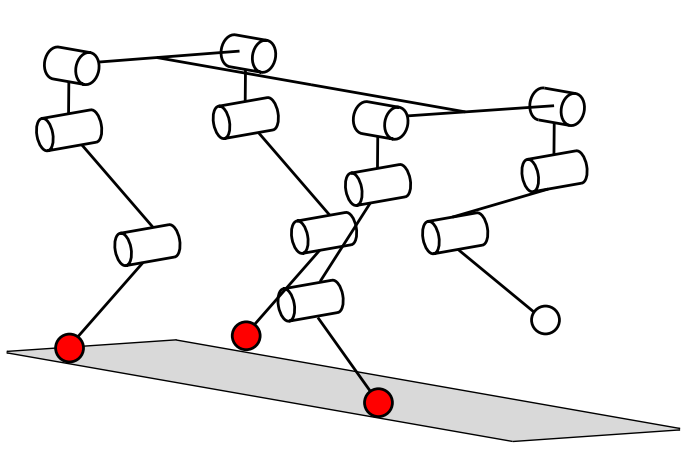
\includegraphics[width=\linewidth]{img/example.png} 

   


%%%%%%%%%%%%%%%%%%%%%%%%%%%%%%%%%%%%%%%%%%%%%%%%%%%%%%%%%%%%%%%%%%%%%%%%%%%%%%%%
%%                            Fin del documento                               %%
%%%%%%%%%%%%%%%%%%%%%%%%%%%%%%%%%%%%%%%%%%%%%%%%%%%%%%%%%%%%%%%%%%%%%%%%%%%%%%%%
\end{multicols*}
\end{document}
